\section{Survey of approximate matching techniques}
The approximate matching problem is, in general, more complicated than the exact matching problem. We can consider exact matching problems as a subset of approximate matching problems with an error of 0. We should note that the problem set will also change a lot if we use a different error metric(such as Levenshtein distance or Hamming distance) or a different model of errors (such as insertion, deletion or transition). The time complexity of many efficient exact matching algorithms that work as simulating DFAs, such as the Knuth--–Morris--–Pratt algorithm, will become exponential as the number of errors grows if we just convert the NFAs that accepts the pattern with errors into DFAs to be applied in these algorithms. 

From now on we denote the pattern string with $pat$ and the text string with $txt$ and the lengths of them are $m$ and $n$ respectively.

\subsection{Dynamic programming}

One of the classical solutions to approximate matching is to use dynamic programming. This method is relatively straightforward and easy to be implemented by programming. It has been proved that if the alphabet is of a constant size, approximate string matching with $k$ errors can be solved in $O(kn)$ time\cite{crochemore-jewels}. The investigation of the theory background is substantial and can be left as future work.

Here we present an idea of how to match a pattern with the Levenshtein distance by dynamic programming. Informally, the Levenshtein distance between two strings is the minimum number of edits(including replacement, insertion, and deletion) that requires to change one string into the other. The problem above can be considered as filling in a matrix of size $m\times n$. In such a matrix, an element [$i$+1,$j$+1] ($i$ and $j$ denote the number of row and column respectively in the matrix) is filled with the value [$i$,$j$] if $pat$[$i$+1] is the same with $txt$[$j$+1]; otherwise the sum of 1 and the minimum of [$i$,$j$],[$i$,$j$+1] and [$i$+1,$j$], which indicates a replacement, a deletion and an insertion respectively. We show an example of such a problem.


\begin{example} \emph{Dynamic programming solving approximate matching with the Levishtein distance of 1 for pattern "abc" and text "abaab".}

\begin{table}[H]
	\centering
\begin{tabular}{|c|c|c|c|c|c|}
	\hline
	\multicolumn{1}{|l|}{}            & \multicolumn{1}{l|}{}    & \multicolumn{1}{l|}{\textbf{a}}   & \multicolumn{1}{l|}{\textbf{b}}   & \multicolumn{1}{l|}{\textbf{a}} & \multicolumn{1}{l|}{\textbf{a}} \\ \hline
	& \textbf{0}               & 1                                 & 2                                 & 3                               & 4                               \\ \hline
	\textbf{a}                        & 1                        & {\color[HTML]{000000} \textbf{0}} & 1                                 & {\color[HTML]{333333} 2}        & {\color[HTML]{333333} 3}        \\ \hline
	\textbf{b}                        & 2                        & 1                                 & \textbf{0}                        & {\color[HTML]{333333} 1}        & {\color[HTML]{333333} 2}        \\ \hline
	{\color[HTML]{333333} \textbf{c}} & {\color[HTML]{333333} 3} & {\color[HTML]{333333} 2}          & {\color[HTML]{32CB00} \textbf{1}} & {\color[HTML]{000000} 1}        & {\color[HTML]{333333} 2}        \\ \hline
\end{tabular}
\end{table}
	\label{fig:dynap}
 \end{example}
If we look at the last row of this matrix, the filled values from left to right show us how the Levenshtein distance changes between the pattern and the text we have read. When we read in the second character of the text, i.e. $b$, a match is found, that is $ab$ matches $abc$ with one error. The numbers in bold show us the path of this match: two diagonal steps with no increase in the value mean two exact matches of a single character (i.e., matches of $a$ and $b$) and one vertical step means an insertion (i.e., insertion of $c$). 

Dynamic programming is simple, practical and easy to be extended to support more functionalities such as specifying the number of each type of errors, which can be implemented by finding a particular path in the matrix as we have shown above. It is likely that our experiment tools such as Python {\tt regex} and $\operatorname{Scan\_for\_matches}$ are based on this method as the time complexity appears close to linear. As there is no documentation or description of what the approximate matching algorithms are used in these tools, this can be left as future work for further investigation.

\subsection{Automaton simulation} \label{survey-NR-grep}
Another classical approach is to use automaton simulation. The algorithm BNDM  (we will explain later) over which NR-grep is built is a simulation of an NFA. 

From the experiment results shown in the previous section, we find NR-grep has the best performance in average in our various test cases. This is not surprising because NR-grep implemented different efficient algorithms for various pattern matching problems as well as a good software design. We present some important techniques of approximate matching as well as efficient matching algorithms that used in NR-grep.

\subsubsection{Bit-parallelism}

From NR-grep's perspective, the patterns are classified into three levels: simple patterns, extended patterns, and regular expressions. Different patterns are applied with different algorithms to ensure that the problem can be solved in the most efficient way. The name of this tool comes from "nondeterministic reverse $grep$", which indicates this tool can simulate NFAs instead of converting them to DFAs. The algorithm of simulating NFAs used in NR-grep is called $\operatorname{Shift-Or}$. This algorithm is based on an approach called $\operatorname{bit-parallelism}$, which takes advantage of the parallelism of bit operations inside a computer word. A variant of $\operatorname{Shift-Or}$ that is easier to explain is $\operatorname{Shift-And}$ algorithm. We first show how this algorithm works. 

Given both the pattern and the text in the alphabet $\Sigma$ with a size $|\Sigma|$, first we build a table $B$ in which for each character in $\Sigma$ stores a bit mask $b_m...b_1$. For a character $char$ in $pat$ with an index $i$ (1-indexed), set the $\operatorname{(m-i-1)}$ bit of the mask in B[$char$]. The following example shows a bit mask table for the pattern "abc".


\begin{example}\emph{The bit mask table for pattern "abc", assuming $\Sigma$ = \{a,b,c,d\}.}

\begin{table}[H]
	\centering
	\begin{tabular}{|c|c|c|c|}
		\hline
		index      & 1                        & 2                        & 3                        \\ \hline
		\textbf{a} & 0                        & 0                        & {\color[HTML]{3531FF} 1} \\ \hline
		\textbf{b} & 0                        & {\color[HTML]{3531FF} 1} & 0                        \\ \hline
		\textbf{c} & {\color[HTML]{3531FF} 1} & 0                        & 0                        \\ \hline
		\textbf{d} & 0                        & 0                        & 0                        \\ \hline
	\end{tabular}
	\label{table-bitmask}
\end{table}
\end{example}

We use a computer word $D = d_m...d_1$ to store the current active state (or the current matching position in the pattern) with an initial value of all bits 0. During the searching process, $D$ is updated with the following formula: 
$$D' \leftarrow ((D << 1) \ | \ 0^{m-1}1) \ \& \ B[t_j]$$
where $t_j$ is the next text character.  When the $d_m$ bit in $D$ is set, we report a match. 

One of the advantages of the $\operatorname{Shift-And}$ algorithm is that it is easy to be extended to handle classes of characters, which is helpful for approximate matching. 
For example, we can now search for the pattern "ab."\footnote{ We use symbol '.' in this report to stand for a wildcard.}, which can be considered as the pattern "abc" allowing at most one replacement error at the third character, by just setting the $\operatorname{(m-3+1)}$ bit of all the characters in the bit mask table, as the following example shows. 

\begin{example}\emph{The bit mask table for pattern "ab."}.
	\begin{table}[H]
		\centering
		\begin{tabular}{|c|c|c|c|}
			\hline
			index      & 1                        & 2                        & 3                        \\ \hline
			\textbf{a} & {\color{red} 1}                   & 0                        & {\color[HTML]{3531FF} 1} \\ \hline
			\textbf{b} &  {\color{red} 1}                    & {\color[HTML]{3531FF} 1} & 0                        \\ \hline
			\textbf{c} & {\color[HTML]{3531FF} 1} & 0                        & 0                        \\ \hline
			\textbf{d} &{\color{red} 1}                    & 0                        & 0                        \\ \hline
		\end{tabular}
		\label{table-bitmask2}
	\end{table}
\end{example}

With this new bit mask table, searching for the pattern "ab.", or more generally a pattern that contains wildcards, will be just the same time complexity as a search for "abc". 
%We can also find that an error of insertion can be dealt with by adding a new row of all 1s in the bit mask table and a deletion is just removing one row. 

\subsubsection{BNDM algorithm}
As we know, many efficient exact pattern matching algorithms, such as the Knuth--–Morris--–Pratt and the Boyer-Moore algorithm, utilize a trick of skipping characters. It is also possible to combine the $\operatorname{bit-parallelism}$ approach with the ability to skip characters to achieve an even more efficient algorithm. This idea is implemented in the $BNDM$ algorithm as we have introduced before. BNDM uses $\operatorname{Shift-Or}$ instead of $\operatorname{Shift-And}$, a variant of $\operatorname{Shift-And}$ that uses the following state updating formula:  
$$ D' \leftarrow  (D \ \& \ B[t_j]) << 1 .$$ The algorithm that is adapted in BNDM for skipping characters is from the Boyer-Moore or the BDM families\cite{crochemore1994text}.


\subsubsection{NFA simulation}
As we have shown above, bit-parallelism can deal with single error efficiently.
Now we present how bit-parallelism can be used to simulate NFAs for approximate matching. 

Consider the pattern "ab" allowing one error; we can build an NFA to simulate it as the follow figure shows.

\begin{figure} [H]
\begin{center}
	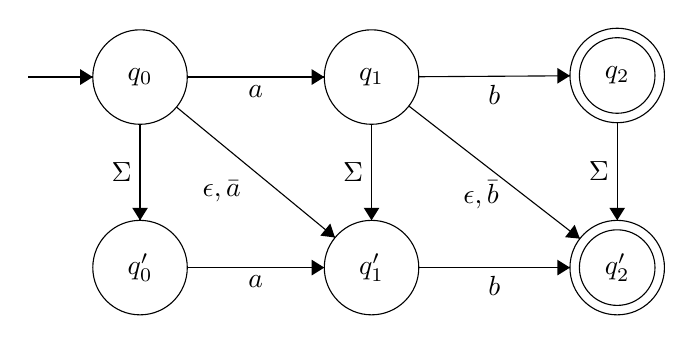
\begin{tikzpicture}[scale=0.2]
	\tikzstyle{every node}+=[inner sep=0pt]
	\draw [black] (18.3,-25.8) circle (3);
	\draw (18.3,-25.8) node {$q_0$};
	\draw [black] (33,-25.8) circle (3);
	\draw (33,-25.8) node {$q_1$};
	\draw [black] (18.3,-37.9) circle (3);
	\draw (18.3,-37.9) node {$q_0'$};
	\draw [black] (33,-37.9) circle (3);
	\draw (33,-37.9) node {$q_1'$};
	\draw [black] (48.6,-25.7) circle (3);
	\draw (48.6,-25.7) node {$q_2$};
	\draw [black] (48.6,-25.7) circle (2.4);
	\draw [black] (48.6,-37.9) circle (3);
	\draw (48.6,-37.9) node {$q_2'$};
	\draw [black] (48.6,-37.9) circle (2.4);
	\draw [black] (11.2,-25.8) -- (15.3,-25.8);
	\fill [black] (15.3,-25.8) -- (14.5,-25.3) -- (14.5,-26.3);
	\draw [black] (21.3,-25.8) -- (30,-25.8);
	\fill [black] (30,-25.8) -- (29.2,-25.3) -- (29.2,-26.3);
	\draw (25.65,-26.3) node [below] {$a$};
	\draw [black] (21.3,-37.9) -- (30,-37.9);
	\fill [black] (30,-37.9) -- (29.2,-37.4) -- (29.2,-38.4);
	\draw (25.65,-38.4) node [below] {$a$};
	\draw [black] (18.3,-28.8) -- (18.3,-34.9);
	\fill [black] (18.3,-34.9) -- (18.8,-34.1) -- (17.8,-34.1);
	\draw (17.8,-31.85) node [left] {$\Sigma$};
	\draw [black] (33,-28.8) -- (33,-34.9);
	\fill [black] (33,-34.9) -- (33.5,-34.1) -- (32.5,-34.1);
	\draw (32.5,-31.85) node [left] {$\Sigma$};
	\draw [black] (36,-25.78) -- (45.6,-25.72);
	\fill [black] (45.6,-25.72) -- (44.8,-25.22) -- (44.8,-26.22);
	\draw (40.8,-26.26) node [below] {$b$};
	\draw [black] (36,-37.9) -- (45.6,-37.9);
	\fill [black] (45.6,-37.9) -- (44.8,-37.4) -- (44.8,-38.4);
	\draw (40.8,-38.4) node [below] {$b$};
	\draw [black] (20.62,-27.71) -- (30.68,-35.99);
	\fill [black] (30.68,-35.99) -- (30.38,-35.1) -- (29.75,-35.87);
	\draw (23.49,-32.34) node [below] {$\epsilon, \bar{a}$};
	\draw [black] (48.6,-28.7) -- (48.6,-34.9);
	\fill [black] (48.6,-34.9) -- (49.1,-34.1) -- (48.1,-34.1);
	\draw (48.1,-31.8) node [left] {$\Sigma$};
	\draw [black] (35.37,-27.64) -- (46.23,-36.06);
	\fill [black] (46.23,-36.06) -- (45.9,-35.18) -- (45.29,-35.97);
	\draw (39.96,-32.35) node [below] {$ \epsilon,\bar{b}$};
	\end{tikzpicture}
\end{center}
\caption{An NFA accepting the pattern "ab" with at most one error.} 
\label{fig:nfa"ab"}
\end{figure}
 
In Figure \ref{fig:nfa"ab"}, the last state of each row stands for a state that accepts $r$ errors where $r$ is the index of the row (0-indexed). That is, in our example, the state $q_2$ accepts "ab" with no errors and $q_2'$  with exact one error: the vertical arrows represent insertions; the diagonal arrows with label $\epsilon$ stand for deletion; the diagonal arrows with $\bar{a}$  \footnote{In this report, we use $\bar{a}$ to denote a symbol $c \in \Sigma \setminus \{a\}$. } stand for replacement for the character $a$. For any other pattern with $k$ errors, we could also build an NFA to accept it in such a way by iteration. It is worth noting that the number of states in the NAF built in this way increases linearly with the number of errors.

The technique stores each row in a machine word, say $R_i$ for row $i$, just as the $D$ we have seen in $\operatorname{Shift-And}$.
The formulas for updating these words are listed below:

\begin{align*}
&R_0' \leftarrow  ((R_0 << 1) \ |\ 0^{m-1}) \ \& \ B[t_j] \\
&for \ i \in 1...k \ do:  \\
&\ \ \ \ R_i' \leftarrow ((R_i << 1) \ \& \ B[t_j] ) \ |\ R_{i-1} \ | \ (R_{i-1} << 1 ) \ |\ (R_{i-1}' << 1)
\end{align*}

These formulas show us one case of how bit-parallelism simulate an NFA. $R_0$ is updated just as we have done with $D$ in $\operatorname{Shift-And}$. In the formula for updating $R_i$, the first element (i.e., $((R_i << 1) \ \& \ B[t_j] ) $ ) is similar to the one for updating $R_0$  but without the $OR$ operation with $0^{m-1}$ because $R_i$ can not be an initial state that has a self-loop. The second is the old value of its upper row, which corresponds to a vertical arrow in the NFA. Similarly, the third stands for a replacement and the fourth a deletion. When we detect that $R_k \& 10^{m-1}$ is not zero, a match is reported.  

As we can see from the above updating formulas, each updating is just bitwise operation hence constant time. So this simulation should be only linear time complexity increased, i.e., $O(k)$, compared with the simulation of exact matching of the same pattern.


\subsubsection{Splitting technique}
An important property of $k$ errors approximate matching has been found that if we split the pattern into $k+1$ pieces, then there must be at least one piece that has no errors\cite{wu1992}. Note that this property only works for an error model of insertion, replacement, and deletion. With this property, the approximate matching problem can be reduced to the multi-pattern matching problem with an extra verification, which is to check if the surrounding text of these pieces can be a match of the whole pattern that allows $k$ errors. This technique is also employed in NR-grep. 
